\autsubsection{Laser Drilling}{Bhaaeddin Alhomsi}

Lasers may provide another method. High-power lasers exceeding 10 kW have been developed and widely used for industry (Gapontsev et al., 2009; Richardson et al., 2010; Fujita et al., 2010). For example, a recent laboratory test using a 1.6-kW pulsed Nd:YAG 1.064 $\mu$m wavelength laser beam determined the energy required to spall, melt, and
vaporize several rock samples for oil and gas well drilling. The required energy (specific energy) depends on the absorption properties of each rock sample as well as the reflective properties of the rock surface  (Gahan and Parker, 2001; Xu et al., 2003). A new laser-mechanical bit for laser spallation of rock to give an optimum drilling mechanism
was found to reduce rig time and increase drilling efficiency (Pooniwala, 2006).More recently, a 20-kWlaserwas delivered through a 1500 m-long optical fiber cable and shown to be able to efficiently drill oil and gas wells (Hecht, 2012). Finally, in the project VALKYRIE,
ice was drilled by a self-contained "intelligent ice penetrator", a 5 kW laser at 1070 nm wavelength (Siegel et al., 2013)(Stone et al., 2014).
Test of VALKYRIE between 2010 and 2013 used high-power optical energy transfer over km-scale distances and tested the feasibility of a vehicle deployed optical waveguide. Thus, a laser-drill system may be useful for ice-sheet applications, including the search for life in extreme environmental conditions here on Earth as well as outer planets.
With continual improvements, laser drilling may develop advantages over other methods for ice.We investigate here the behaviour of laser melting of ice and snow with an infrared laser for the potential use as a drill. We use a $CO_2$ laser, which is a relatively inexpensive
common infrared gas laser (Patel, 1964) with fundamental lines from 9.2 to 10.8 $\mu$m and used in both pulse and continuous wave (CW) mode. For ice, an earlier study demonstrated the potential of $CO_2$ laser irradiation to help breakup nautical sea-ice (Clark et al.,  1973), but the laser has apparently not previously been used for snow
and ice drilling.

\subsubsection{Characteristics of light absorbance in ice}

The absorption of light in ice depends on the complex refractive index of ice. According to data in a previous study (Warren and Brandt, 2008), the absorption coefficient of ice significantly increases from the near- to mid-infra-red region, reaching a value of about $\unit[628.3]{cm^{-1}}$ at the $CO_2$ laser wavelength of 10.6 $\mu$m. Ice absorbs almost 100\% of the light intensity at 10.6 and 1.064 $\mu$m within a penetration distance of 0.01 and 2 cm, as shown in Figure \ref{fig:bh1}.

\begin{figure}[htb]
\centering
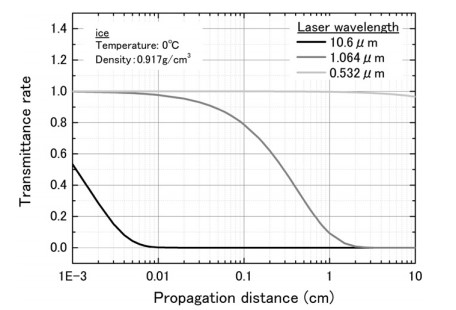
\includegraphics[scale=1]{figures/laser-drilling/bh1.jpg}
\caption{Characteristics of light absorbance in ice}
\label{fig:bh1}
\end{figure}

\subsubsection{Melting studies of ice and snow by $CO_2$ laser}

A $CO_2$ laser can be used to melt ice. The $CO_2$ laser at 10.6 $\mu$m (25.5 W) and a beam diameter of 1.0 cm, a wavelength at which ice strongly absorbs, to drill (via melting) through ice. The resulting drilling speed is measured at several irradiation intensities, ice-snow densities, and beam angles relative to the horizontal axis.
The melting speed increases with increasing laser intensity and with decreasing ice density, as shown in Figure \ref{fig:bh2}. The melting speed ratio between ice ($\unitfrac[917]{kg}{m^3}$) and the lowest-density snow ($\unitfrac[153]{kg}{m^3}$) is 4-5, slightly less than the value of \~6 expected from the density ratio. The reason for this discrepancy could be explained by the snow having a greater reflectivity than solid ice. The melting speed decreases with increasing snow density.

\begin{figure}[htb]
\centering
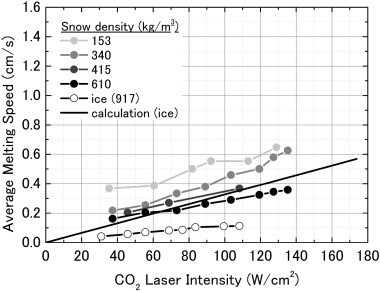
\includegraphics[scale=1]{figures/laser-drilling/bh2.jpg}
\caption{Relation between laser intensity and melting speed}
\label{fig:bh2}
\end{figure}

\subsubsection{Results}

Unfortunately, the experimental results indicate that the melt-water accumulates in the hole and reduces the melting speed of ice and a pump system could not be installed due to a high distance.
In future studies, it will be necessary to investigate quantitatively several additional factors. These include 1) the optical-fiber coupled laser intensities required for deep drilling, 2) a method to pump melted water  Despite these hurdles, the present study suggests that a laser-drilling system could be a new and promising technology.
